\documentclass[9pt]{beamer}

\usepackage[utf8]{inputenc}
%\usepackage{bookman}
\usetheme{Copenhagen}
\usecolortheme{seahorse}
\usepackage{amsmath}
\usepackage{amsthm}
\usepackage{amsfonts}
\usepackage{color}
\usepackage{graphicx}
\usepackage{subcaption}
\usepackage{wrapfig}
\newtheorem{remark}{Remark}[]
\newtheorem{prop}{Properties}
\newtheorem{theor}{Theorem}
\usepackage{amssymb}
\usepackage{enumitem}
\usepackage{tikz}
\usepackage{smartdiagram}
\usepackage{hyperref}
\usepackage{array}

\newcommand{\R}{\mathbb{R}}
\newcommand{\C}{\mathbb{C}}
\newcommand{\N}{\mathbb{N}}
\newcommand{\Q}{\mathbb{Q}}
\newcommand{\W}{\mathbb{W}}
\newcommand{\Vspace}{\mathbb{V}}
\newcommand{\Hspace}{\mathbb{H}}
\newcommand{\Lspace}{\mathbb{L}}
\newcommand{\Lagr}{\mathcal{L}}
\newcommand{\Cmod}{\mathcal{C}}

\DeclareMathOperator*{\argmin}{argmin}
%Information to be included in the title page:
\title[Linear Elasticity]{Linear Elasticity Modelling in 2D and 3D\\ Using Finite Element Method}
\author[Alifian]{Alifian Mahardhika Maulana}
\institute{Kanazawa University}
\date[KU 2018]{2018}



\begin{document}
\frame{\titlepage}

\begin{frame}
\frametitle{Table of Contents}
\tableofcontents
\end{frame}

\begin{frame}{Basic Theory}
We define:
\begin{equation*}
\begin{aligned}
&\Omega \subset \R^d\ (d=2,3)\\
&u:\Omega \rightarrow \R^d\ \text{(displacement)}\\
&e[v]:= \frac{1}{2}(\triangledown^T v + \triangledown v^T)\ \text{(strain)}\\
&\triangledown^T v := \begin{pmatrix}
\partial_1 v_1 & \partial_2 v_2\\
\partial_1 v_2 & \partial_2 v_1
\end{pmatrix}\\
& \triangledown v^T := ( \triangledown^T v)^T\\
&\sigma[u]:=\Cmod e[u]\\
&\Cmod=(C_{ijkl})\begin{cases}
C_{ijkl}=C_{klij}=C_{jikl}\\
(C_\xi):\xi \geq C_* |\xi|^2 (\forall \xi \in \R_{sym}^{d\times d})
\end{cases}
\end{aligned}
\end{equation*}
\end{frame}

\begin{frame}{Linear Elasticity Problem}
\begin{equation}\label{linearelcase}
(**)\begin{cases}
-div\ \sigma[u]=f(x),\ \text{in}\ \Omega\\
u=g(x)\ \text{on}\ \Gamma_D\\
\sigma[u] \nu = q(x)\ \text{on}\ \Gamma_N
\end{cases}
\end{equation}
\begin{equation*}
f \in L^2(\Omega : \R^d,\ g\in H^1(\Omega : \R^d),\ q\in L^2(\Gamma_N:\R^d))
\end{equation*}
\end{frame}

\begin{frame}{Strong Solution $\iff$ Weak Solution}
\begin{equation*}
u\in H^2 (\Omega : \R^d)\ \text{satisfies}\ (**)\ \text{then we call $u:$ a strong solution}
\end{equation*} \centering $\Updownarrow$ \begin{equation*}
\begin{cases}
\int_\Omega \sigma[u] : e[v] dx = \int_\Omega f\cdot v dx + \int_{\Gamma_N} q\cdot v ds\\ \big( \forall v \in V:= \{ v \in H^1\ (\Omega : \R^d)\ |v|_{\Gamma_D} = 0 \}\big)\\
u \in V+g
\end{cases}
\end{equation*}
\end{frame}

\begin{frame}{Proof of Strong Solution $\iff$ Weak Solution}
\begin{proof}
	($\Rightarrow$)
	Assume we choose $v \in V:= \{ v \in H^1\ (\Omega : \R^d)\ |v|_{\Gamma_D} = 0 \}$, with $v$ is a very smooth test function. Then we take integral over the domain for equation \eqref{linearelcase} on both side.
	\begin{equation*}
	\begin{aligned}[center]
	\int_\Omega -div\sigma[u] \cdot v dx &= \int_\Omega f \cdot v dx\\
	\int_\Omega \sigma[u] : \triangledown v dx - \int_\Gamma \sigma[u]\nu \cdot v ds &= \int_\Omega f \cdot v dx\\
	\int_\Omega \sigma[u] : \triangledown v dx - \bigg(\int_{\Gamma_D} \sigma[u]\nu \cdot v ds + \int_{\Gamma_N} \sigma[u]\nu \cdot v ds\bigg) &= \int_\Omega f \cdot v dx\\	
	\end{aligned}
	\end{equation*}
	From Boundary Condition we know that:
	\begin{equation*}
	\begin{cases}
	v = 0\ \text{on}\ \Gamma_D\\
	\sigma[u] \nu = q\ \text{on}\ \Gamma_N
	\end{cases}
	\end{equation*}
\end{proof}
\end{frame}

	\begin{frame}
	\begin{proof}
	Hence, we have:
	\begin{equation}\label{weakproof}
	\begin{aligned}[center]
	\int_\Omega \sigma[u] : e[v] dx - \int_{\Gamma_N} q \cdot v ds &= \int_\Omega f \cdot v dx\\
	\int_\Omega \sigma[u] : e[v] dx &= \int_\Omega f \cdot v dx + \int_{\Gamma_N} q \cdot v ds \\
	\end{aligned}
	\end{equation}
	with:
	\begin{equation*}
	\begin{aligned}
	&X:= H^1(\Omega : \R^d)\\
	&a(u,v) := \int_\Omega \sigma[u] : e[v] dx\\
	&l(v) := \int_\Omega f\cdot v dx + \int_{\Gamma_N} q \cdot v ds\\
	\end{aligned}
	\begin{aligned}
	a(u,v) &= \int_\Omega (\Cmod e[u]) : e[v] dx\\
	&= \int_\Omega e[v] : (\Cmod e[u]) dx\\
	&= a(v,u)
	\end{aligned}
	\end{equation*}
	Then we rewrite equation \eqref{weakproof} in a bilinear and linear form:
	\begin{equation*}
	a(u,v) = l(v)
	\end{equation*}
\end{proof}
\end{frame}

\begin{frame}{Modelling and Simulation}
In this simulation, we use a cantilever beam (Mild Steel Material) as the domain, which is a thin rectangular cross section introduced by Timoshenkol Goodier (1970), then we must specify nondimensionalized value for simulation as shown in table \ref{parametertable}.
\begin{table}[h!]
	\centering
	\begin{tabular}{|l|l|l|}
		\hline
		Numerical Parameter & Typical Value [unit] & Nondimensionalized value\\
		\hline
		Young's modulus (E) & $2.1 \times 10^7$ [Pa] & 210\\
		Poisson's ratio ($\nu$) & 0.3 [-] & 0.3\\
		Gravity constant (f) & 9.80655 [N/kg] & 9.80655\\
		Weight (q) & 0 [N] & 0\\
		Length (L) & 3.0 [m] & 3.0\\
		Depth (h) & 0.2 [m] & 0.2\\
		Width (b) & 0.25 [m] & 0.25\\
		\hline
	\end{tabular}
	\caption{Material properties and numerical parameters}
	\label{parametertable}
\end{table}
\end{frame}

\begin{frame}
\begin{figure}[h!]
	\centering
	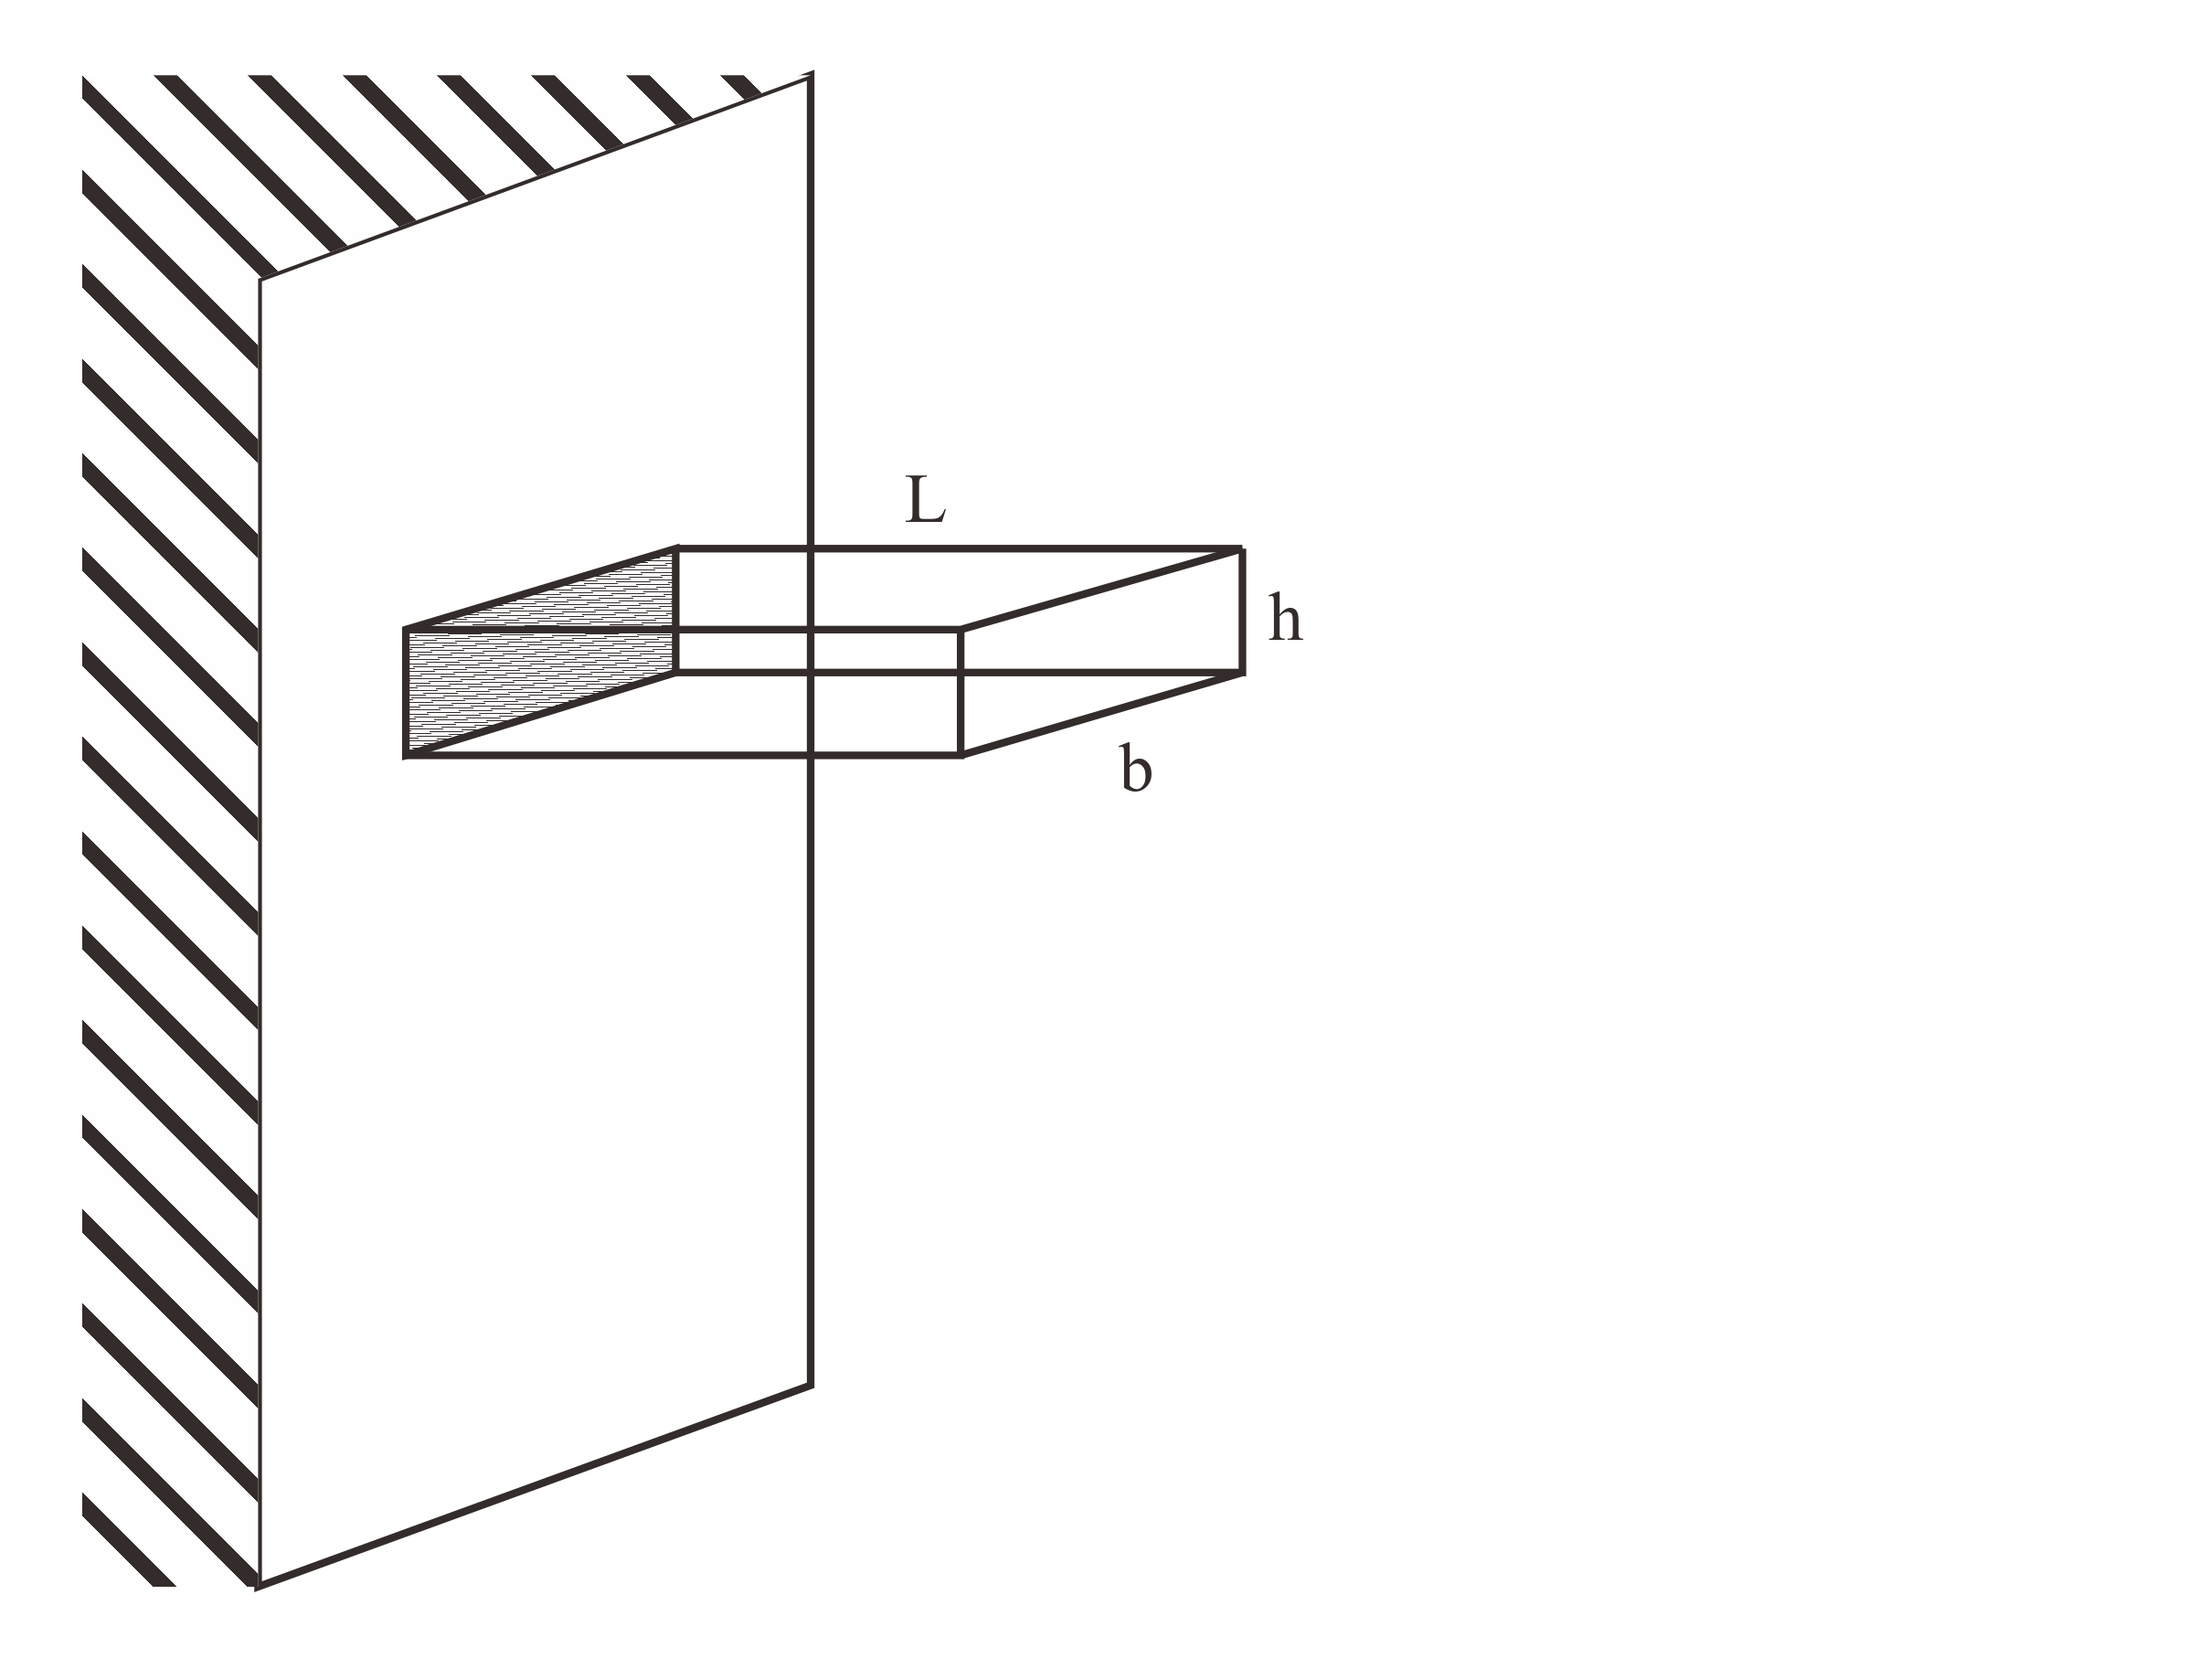
\includegraphics[width=0.5\linewidth]{picture/3dmodellinearelasticity}
	\caption{3D Model of cantilever beam. We use gravity force as the body force \textbf{f} and fixed the left part of the beam, and then we give a 1 Newton weight force act on the right part of the beam as the neumann boundary condition \textbf{q}.}
	\label{fig:3dmodel}
\end{figure}
\end{frame}

\begin{frame}
With the help of FreeFem++ software, we created a 2D and 3D model as shown in figure \ref{fig:3dmodel}, then we solve the displacement vector ($u$, $v$) after solving the displacement, we calculate $\sigma$ which stand for stress force acting on surface of the cantilever beam using equation below:
\begin{equation*}
\begin{aligned}[center]
\sigma = (d \lambda^2 + 4\lambda\mu)div(u)^2 + (4\mu^2 |e[u]|^2),\ d=2,3\\
\lambda\ \text{(Lame's first parameter)}\ := \frac{E\nu}{(1+\nu)(1-2\nu)}\\
\mu\ \text{Lame's second parameter}\ := \frac{E}{2(1+\nu)}
\end{aligned}
\end{equation*}
\end{frame}

\begin{frame}{Result and Discussion}
The simulation used mesh P1 finite element method on FreeFEM++, where $u$ and $v$ calculated for division number of mesh equal 16. In the figure \ref{fig:displacementresult} we can see the deformation of the cantilever beam in 2D and 3D graphics.
\begin{figure}[h!]
		\centering
		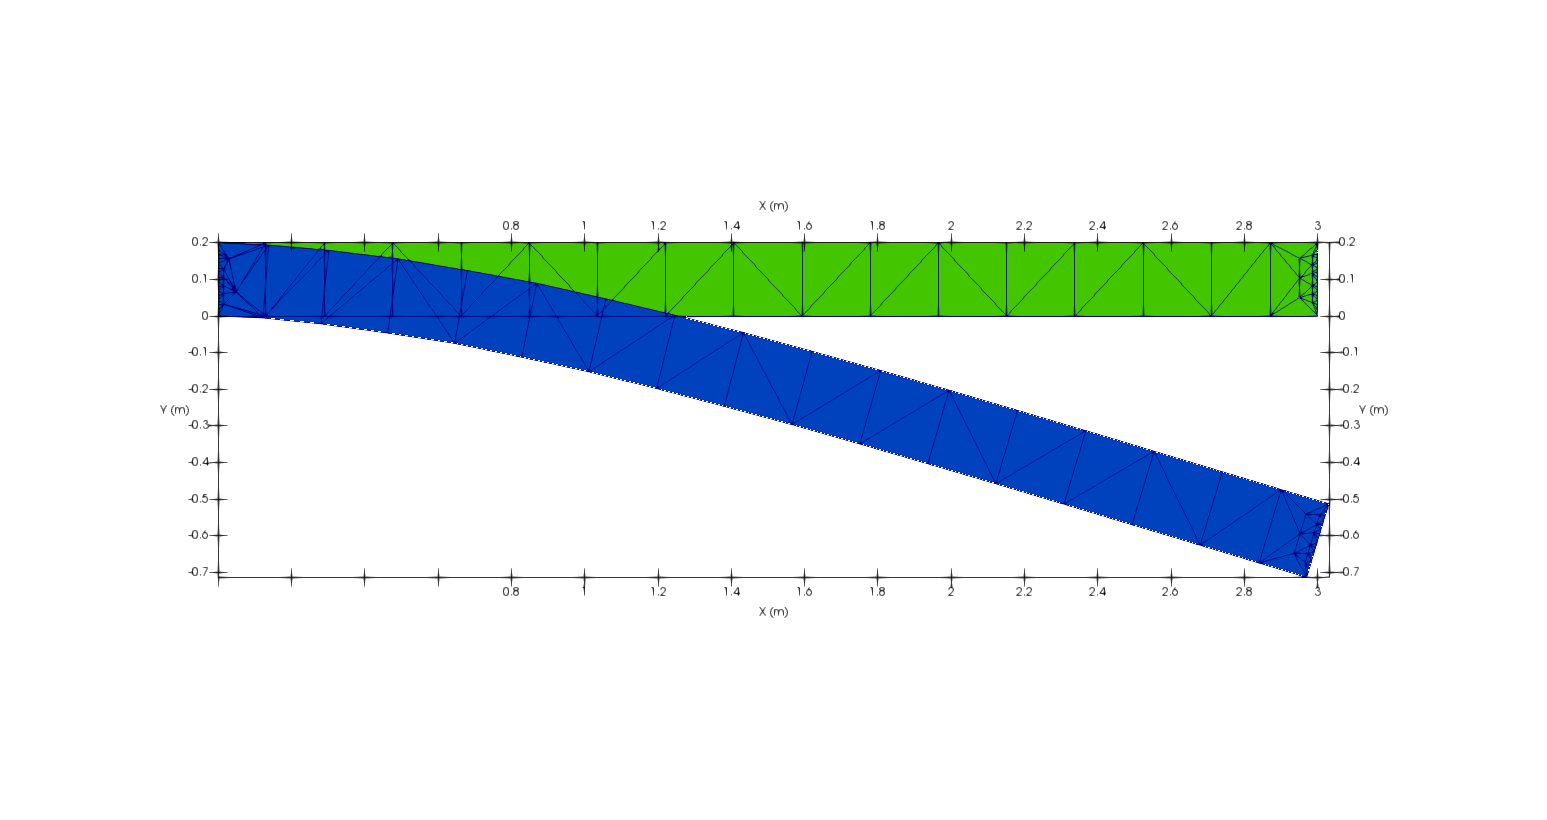
\includegraphics[width=\linewidth]{picture/conference/2d1}
		\caption{Deformation in 2D. Green line show condition before gravity and weight force applied to the domain. Red line show condition after we solve linear elasticity with gravity and weight force applied to the domain. Maximal Displacement ($u = 0.03\ [m]$)}
		\label{fig:2dresult}
\end{figure}
\end{frame}
\begin{frame}
\begin{figure}[h!]
	\centering
	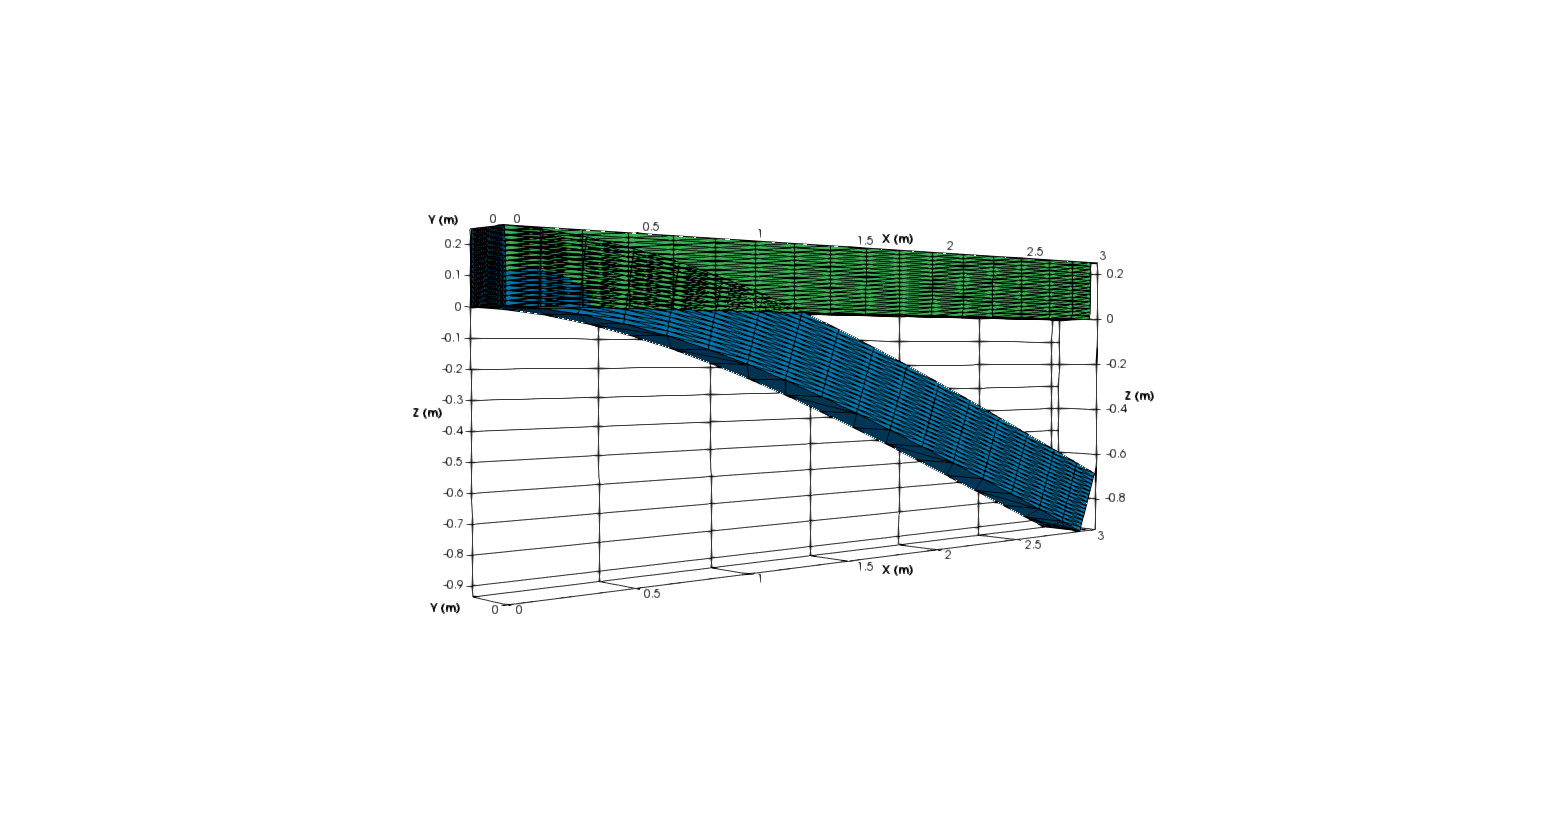
\includegraphics[width=\linewidth]{picture/conference/3d1}
	\caption{Deformation in 3D. Green line show condition before gravity and weight force applied to the domain. Red line show condition after we solve linear elasticity with gravity and weight force applied to the domain. Maximal Displacement ($u = 0.05\ [m]$)}
	\label{fig:3dresult}
\end{figure}
\end{frame}
\begin{frame}
While in the figure \ref{fig:2dstress} we can see result from calculating the stress tensor on 2D and 3D case.
\begin{figure}[h!]
		\centering
		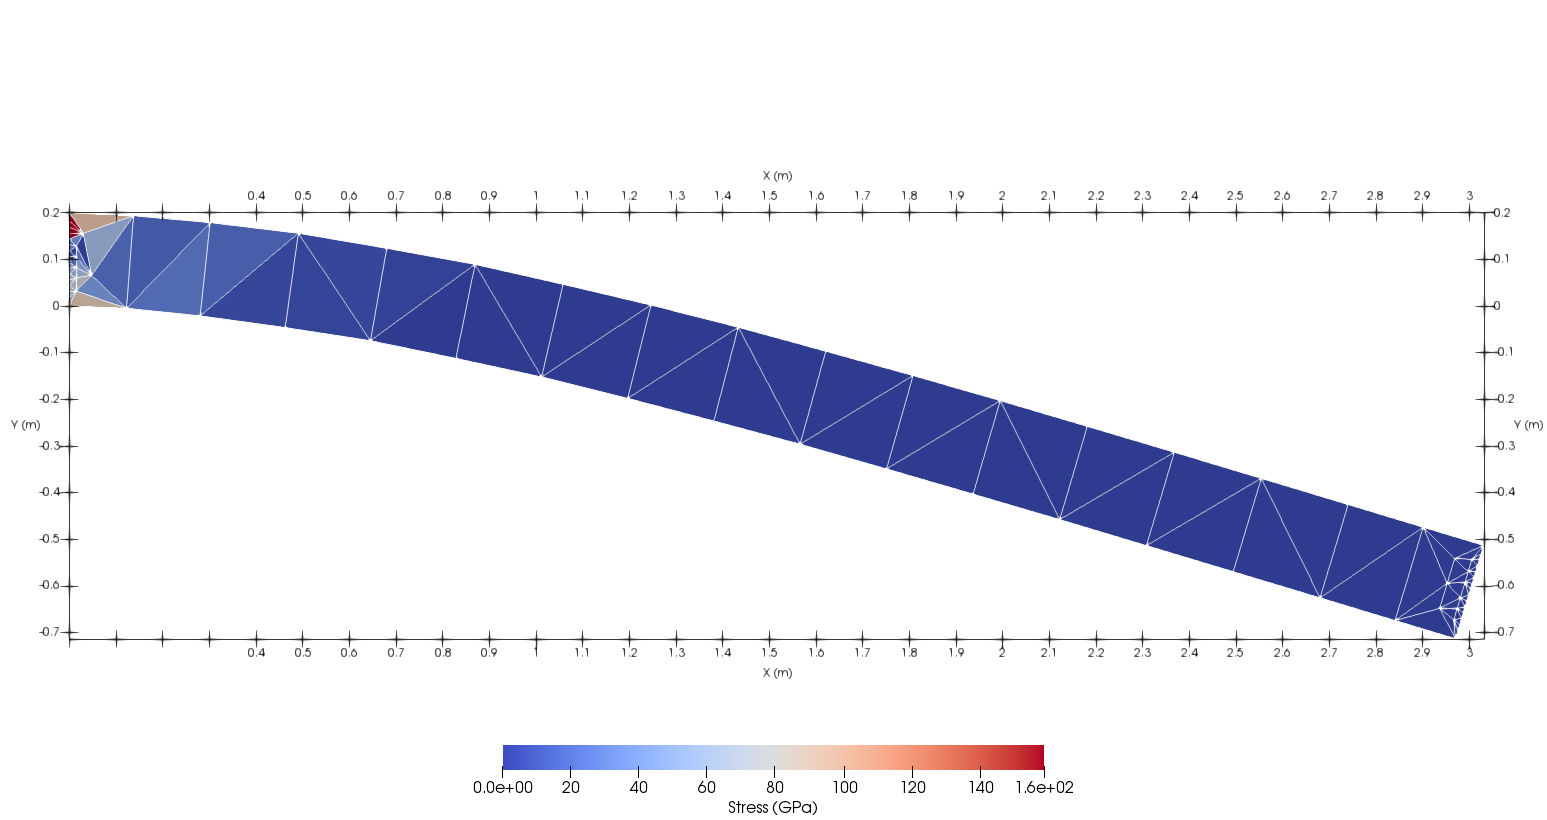
\includegraphics[width=\linewidth]{picture/conference/2dstress}
		\caption{Calculated $\sigma$ on 2D case. The value of $\sigma$ on the domain, maped by the color in the picture with respect to the color palette on the lower side of the graph. Maximal stress given on the surface ($\sigma = 158.612\ [GPa]$)}
		\label{fig:2dstress}
\end{figure}
\end{frame}
\begin{frame}
\begin{figure}[h!]
	\centering
	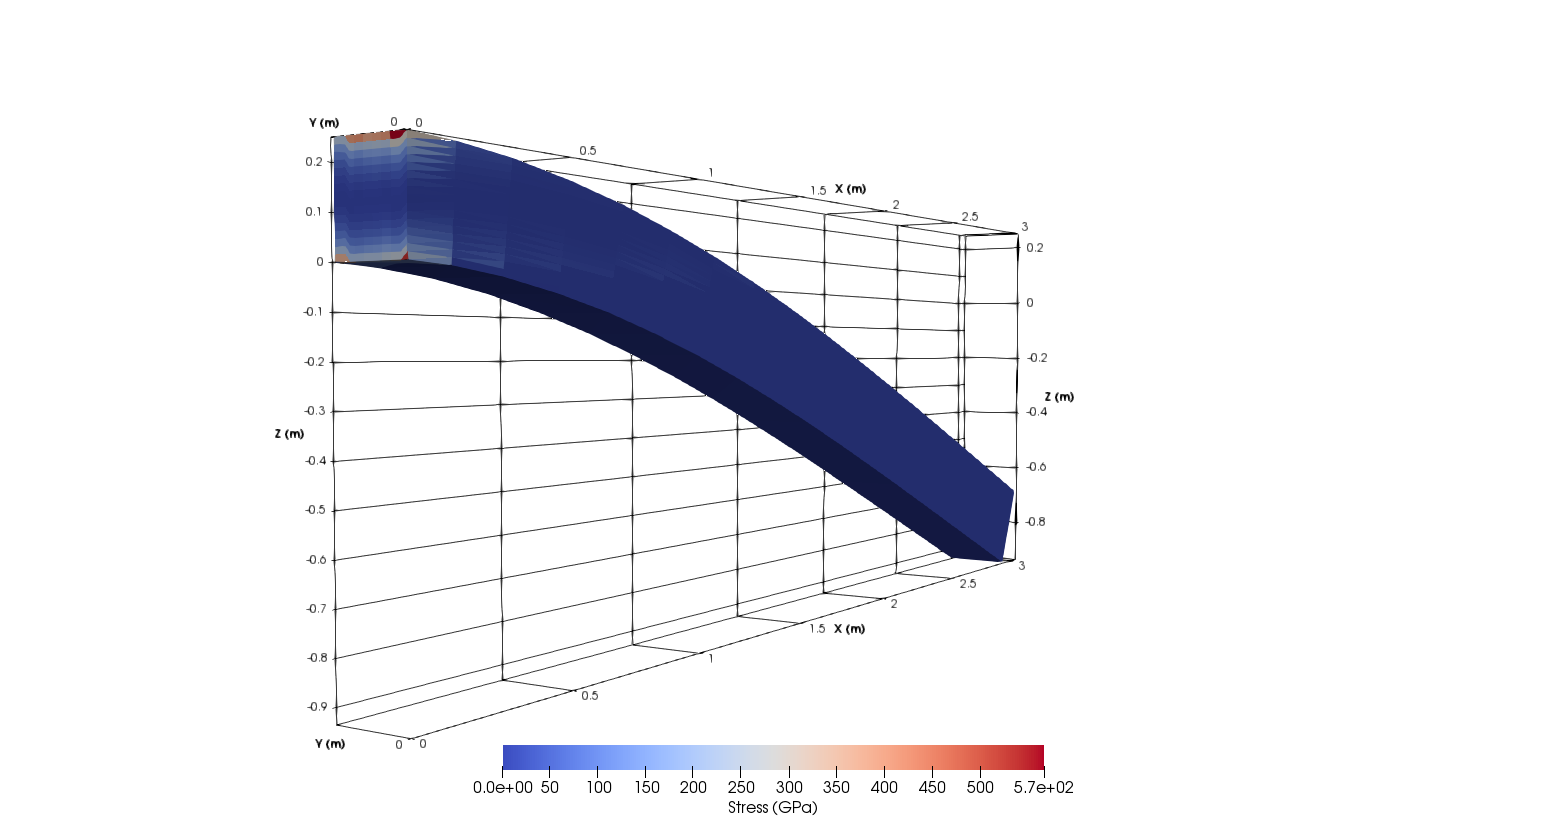
\includegraphics[width=\linewidth]{picture/conference/3dstress}
	\caption{Calculated $\sigma$ on 3D case. The value of $\sigma$ on the domain, maped by the color in the picture with respect to the color palette on the lower side of the graph. Maximal stress given on the surface ($\sigma = 567.034\ [GPa]$)}
	\label{fig:3dstress}
\end{figure}
\end{frame}
\end{document}